\chapter{Divergences and Dual Norms}

\index{dual!norm}% strictindex
\label{sec-divergences-dual-norms}


This chapter compares OT with divergence-based and adversarial ways of measuring discrepancy. The central issue is topological: $\phi$-divergences are cheap but strong, while dual norms and GAN objectives can be weak enough to compare singular measures. The discussion connects classical information divergences~\cite{ciszar1967information,ali1966general} with modern integral probability metrics and generative modeling~\cite{sriperumbudur2009integral,GAN,WassersteinGAN}.
\index{generative model}% strictindex
\index{integral probability metric}% strictindex
\index{phi-divergence}% strictindex

%%%%%%%%%%%%%%%%%%%%%%%%%%%%%%%%%%%%%%%%%%%%%%%%%%%%%%%%%%%%%%%%%%%%%%%%
\section{Dual norms (Integral Probability Metrics)}
\index{dual!norm}% strictindex
\label{sec-dual-norms}

This section isolates the test-function viewpoint behind weak discrepancies. Dual norms generalize the $\Wass_1$ test-function principle. They are useful in statistics because they compare distributions by restricting the discriminator class.
\index{dual!norm}% strictindex
\index{discriminator class}% strictindex

\paragraph{Integral probability metrics.}
\index{integral probability metric}% strictindex

Formulation~\eqref{eq-w1-cont} is a special case of a dual norm. This viewpoint provides a way to design ``weak'' discrepancies by testing signed differences of measures against a controlled class of functions.
\index{measurable function}% strictindex
\index{dual!norm}% strictindex

\begin{defn}[Dual seminorm and integral probability metric]\label{def-dual-norm-ipm}
	Let $B$ be a nonempty symmetric convex class of measurable functions that are integrable against the measures under consideration. For a signed measure $\xi$, define the extended dual seminorm
	\eql{\label{eq-dual-norm-cont}
		\norm{\xi}_B \eqdef
		\usup{\f} \enscond{ \int_{\Xx} \f(x) \d\xi(x) }{ \f \in B}.
	}
	It is a norm when it is finite and $B$ separates signed measures. When applied to $\al-\be$ for probability measures, it is called an integral probability metric (IPM); it is a genuine metric precisely when $B$ separates probability measures.
\end{defn}
Symmetry makes the supremum equal to $\sup_{f\in B}|\int f\d\xi|$, while convexity makes $B$ a natural unit ball. The choice of $B$ determines both the topology and the statistical behavior of the discrepancy; see~\cite{sriperumbudur2012empirical,sriperumbudur2009integral,sriperumbudur2008injective}.
\index{integral probability metric}% strictindex
\index{dual!norm}% strictindex

\begin{example}[Total variation]
\index{total variation}% strictindex
As recalled in Definition~\ref{defn-total-variation} and Proposition~\ref{prop-tv-dual-measure}, total variation is the dual norm associated with the unit ball of continuous functions
\eq{
	B = \enscond{f \in \Cc(\Xx)}{\norm{f}_\infty \leq 1}.
}
Total variation is the canonical nontrivial example of a discrepancy that is both a $\phi$-divergence and a dual norm; see~\cite{sriperumbudur2009integral}.
\index{phi-divergence}% strictindex
\index{dual!norm}% strictindex
\end{example}

\begin{example}[$\Wass_1$ norm]
On zero-mass signed measures with finite first moment, the Kantorovich--Rubinstein norm underlying $\Wass_1$, as defined in~\eqref{eq-w1-cont}, is the extended dual seminorm~\eqref{eq-dual-norm-cont} associated with
\eq{
	B = \enscond{f}{\Lip(f) \leq 1}
}
the set of 1-Lipschitz functions.
\index{Lipschitz!function}% strictindex
\end{example}

\begin{example}[Flat norm and Dudley metric]
\index{norm!flat}% strictindex
\index{Dudley metric}% strictindex
If $B$ is uniformly bounded and separates measures, then $\norm{\cdot}_B$ is a finite norm on the whole space $\Mm(\Xx)$ of finite signed measures.
\index{finite measure}% strictindex
%
This is not the case for $\Wass_1$: zero total mass, $\xi(\Xx)=0$, is necessary, and on an unbounded space one also needs a finite first moment. If the mass is nonzero, $\norm{\xi}_B=+\infty$ because constants belong to the Lipschitz ball.
%
This is remedied by imposing a bound on the value of the potential $\f$, which leads for instance to the flat norm,

\eql{\label{eq-set-flatnorm}
	B=\enscond{f}{\Lip(f) \leq 1 \qandq \norm{\f}_\infty \leq 1}.
}
On compact metric spaces, it metrizes weak convergence of finite nonnegative measures, and more generally weak-* convergence on every total-variation-bounded subset of $\Mm(\Xx)$.
\index{finite measure}% strictindex
\index{weak!convergence}% strictindex
%
The finite-dimensional version is obtained from the usual $\Wass_1$ dual linear program by adding the box constraints $\abs{\fD_k}\leq1$.
%
The flat norm is sometimes called the ``Kantorovich--Rubinstein'' norm~\cite{hanin1992kantorovich} and has been used as a fidelity term for inverse problems in imaging~\cite{lellmann2014imaging}.
\index{norm!flat}% strictindex
%
The flat norm is equivalent to the bounded-Lipschitz, or Dudley, metric, whose test class is
\index{Dudley metric}% strictindex
\eq{\label{eq-set-dudley}
	B=\enscond{f}{\Lip(f) + \norm{f}_\infty \leq 1}.
}
On a Euclidean domain, $\Lip(f)=\norm{\nabla f}_\infty$ for differentiable $f$.
\end{example}

Figure~\ref{fig:dualnorms-ipm-witnesses} compares the optimal test functions selected by several integral probability metrics for the same pair of one-dimensional densities.

\begin{figure}[ht]
\centering
\setlength{\tabcolsep}{2pt}
\begin{tabular}{@{}ccc@{}}
\small $\Wass_1$ witness & \small MMD witness & \small total variation witness \\[-.15em]
\index{total variation}% strictindex
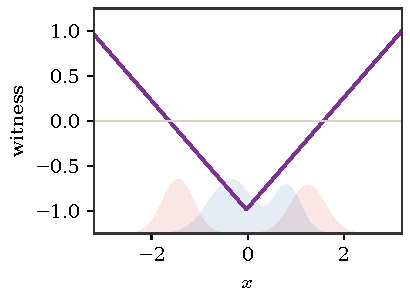
\includegraphics[width=.31\linewidth]{figures/dualnorms-ipm-witnesses/w1.pdf} &
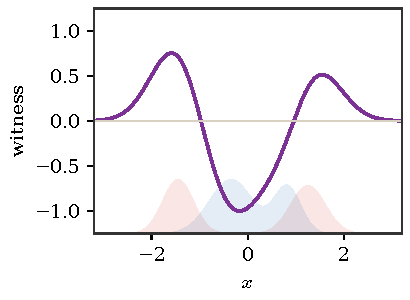
\includegraphics[width=.31\linewidth]{figures/dualnorms-ipm-witnesses/mmd.pdf} &
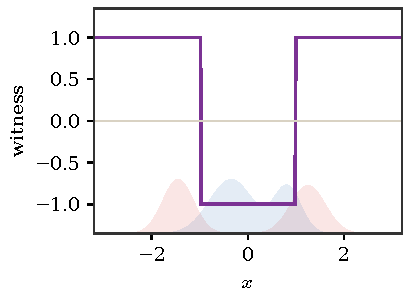
\includegraphics[width=.31\linewidth]{figures/dualnorms-ipm-witnesses/tv.pdf}
\end{tabular}
\caption{\emph{Dual witnesses for integral probability metrics.} The red and blue curves are two one-dimensional probability densities and the violet curve is a normalized optimal dual witness $f^\star_{\alpha,\beta}$ for the IPM variational problem~\eqref{eq-dual-norm-cont}. $\Wass_1$ restricts the slope through Kantorovich--Rubinstein duality~\eqref{eq-w1-cont}, MMD restricts the RKHS norm as in Proposition~\ref{prop-kernel-rkhs-dual}, and total variation can saturate pointwise and therefore reacts sharply to signed density differences.}
\index{Kantorovich-Rubinstein@Kantorovich--Rubinstein!duality}% strictindex
\index{integral probability metric}% strictindex
\index{dual!norm}% strictindex
\index{RKHS}% strictindex
\index{maximum mean discrepancy}% strictindex
\label{fig:dualnorms-ipm-witnesses}
\end{figure}

The following proposition gives a useful compact-space criterion. The dual ball should be rich enough to approximate continuous observables, but compact enough for weak convergence to imply uniform convergence over the discriminator class.
\index{discriminator class}% strictindex
\index{weak!convergence}% strictindex

\begin{prop}[Metrization by dual norms]\label{prop-dual-norm-metrization}
\index{dual!norm}% strictindex
	Assume that $\Xx$ is compact, that $B=-B$, and that the measures considered are probability measures.
\index{probability measure}% strictindex
	\begin{enumerate}
		\item If every function in $\Cc(\Xx)$ can be uniformly approximated by elements of $\Span(B)$, then $\norm{\al_n-\al}_B \rightarrow 0$ implies $\al_n \rightharpoonup \al$.
		\item If $B \subset \Cc(\Xx)$ is compact for $\norm{\cdot}_\infty$, then $\al_n \rightharpoonup \al$ implies $\norm{\al_n-\al}_B \rightarrow 0$.
	\end{enumerate}
\end{prop}
\begin{proof}
	For the first implication, $\norm{\al_n-\al}_B\to0$ and the symmetry of $B$ imply
	\[
		\abs{\dotp{f}{\al_n-\al}}\leq \norm{\al_n-\al}_B
		\qforq f\in B.
	\]
	If $h=\sum_{j=1}^J c_j f_j\in\Span(B)$, then
	\[
		\abs{\dotp{h}{\al_n-\al}}
		\leq \pa{\sum_{j=1}^J|c_j|}\norm{\al_n-\al}_B,
	\]
	so integrals converge for every $h\in\Span(B)$. Let $u\in\Cc(\Xx)$ and choose such an $h$ with $\norm{u-h}_\infty\leq\eta$. Since $\al_n$ and $\al$ are probabilities,
	\[
		\abs{\dotp{u}{\al_n-\al}}
		\leq
		\abs{\dotp{h}{\al_n-\al}}+2\eta.
	\]
	Taking the limsup as $n\to\infty$ and then letting $\eta\to0$ gives $\dotp{u}{\al_n}\to\dotp{u}{\al}$ for all $u\in\Cc(\Xx)$, which is weak convergence.
\index{weak!convergence}% strictindex

	For the second implication, assume $\al_n\rightharpoonup\al$ and choose a subsequence $(\al_{n_k})_k$ such that $\norm{\al_{n_k}-\al}_B\to\limsup_n\norm{\al_n-\al}_B$. Since $B$ is compact and the map $f\mapsto\dotp{f}{\al_{n_k}-\al}$ is continuous on $B$, the supremum is attained by some $f_{n_k}\in B$. Extracting a further subsequence if needed, $f_{n_k}\to f$ uniformly for some $f\in B$. Then
	\[
		\dotp{f_{n_k}}{\al_{n_k}-\al}
		=
		\dotp{f}{\al_{n_k}-\al}
		+\dotp{f_{n_k}-f}{\al_{n_k}}
		-\dotp{f_{n_k}-f}{\al}.
	\]
	The first term tends to zero by weak convergence and the last two by uniform convergence. Hence every limsup subsequence has limit zero, proving $\norm{\al_n-\al}_B\to0$.
\index{weak!convergence}% strictindex
\end{proof}

\begin{cor}[Wasserstein metrizes weak convergence]\label{cor-topol-wass}
	On a compact metric space, $\Wass_p$ metrizes weak convergence on probability measures for every $p\geq1$.
\index{probability measure}% strictindex
\end{cor}
\begin{proof}
	For $p=1$, take $B=\enscond{f}{\Lip(f)\leq1}$. The span of $B$ contains all Lipschitz functions, and Lipschitz functions are dense in $\Cc(\Xx)$ on compact metric spaces. This gives the implication $\Wass_1(\al_n,\al)\to0\Rightarrow \al_n\rightharpoonup\al$ by Proposition~\ref{prop-dual-norm-metrization}.
\index{Lipschitz!function}% strictindex
\index{dual!norm}% strictindex

	Conversely, constants do not change the pairing with $\al_n-\al$. Fix $x_0\in\Xx$ and normalize potentials by $f(x_0)=0$. The normalized unit Lipschitz ball is uniformly bounded by $\mathrm{diam}(\Xx)$ and equicontinuous, hence compact in $\norm{\cdot}_\infty$ by Arzel\`a--Ascoli. Proposition~\ref{prop-dual-norm-metrization} gives $\Wass_1(\al_n,\al)\to0$. Proposition~\ref{prop-comp-wass-p} shows that all $\Wass_p$ distances induce the same topology on a compact space, so the result follows for every $p\geq1$.
\end{proof}

\section{Dual RKHS Norms and Maximum Mean Discrepancies}
\index{maximum mean discrepancy}% strictindex
\index{RKHS}% strictindex
\index{reproducing kernel Hilbert space}% strictindex
\label{sec-rkhs-mmd}

Kernel methods turn probability measures into mean elements of a reproducing kernel Hilbert space (RKHS). The resulting Hilbertian dual seminorms are quadratic discrepancies, handled with Euclidean geometry while retaining a weak test-function interpretation. We first recall the positivity assumptions under which the quadratic form on signed measures is nonnegative.
\index{probability measure}% strictindex
\index{signed!measure}% strictindex
\index{dual!norm}% strictindex

\begin{defn}[Positive and conditionally positive kernels]\label{def-positive-kernels}
\index{kernel!positive}% strictindex
\index{conditionally positive kernel}% strictindex
	A symmetric function $\Krkhs:\Xx\times\Xx\to\RR$ is positive definite if for every $n\geq1$, every $x_1,\ldots,x_n\in\Xx$ and every $r\in\RR^n$,
\index{RKHS}% strictindex
	\eql{\label{eq-dual-kern}
		\sum_{i,j=1}^n r_i r_j \Krkhs(x_i,x_j)\geq0.
	}
	It is conditionally positive definite if the same inequality is required only for zero-sum vectors, $\dotp{r}{\ones_n}=0$.
\end{defn}
Here ``positive definite'' is used in the standard kernel-theory sense of positive semidefinite; strict positivity is an additional property. This distinction matters because a non-strict kernel can induce a degenerate discrepancy.

The conditional version is the right notion for probability distances, because one applies the quadratic form to signed measures $\xi=\al-\be$ of total mass zero. Adding a term of the form $a(x)+a(y)$ to the kernel does not change $\iint \Krkhs(x,y)\d\xi(x)\d\xi(y)$ on such measures, and many natural distance kernels are only conditionally positive definite.
\index{signed!measure}% strictindex

\begin{example}[Riesz, energy and Mat\'ern-type kernels]
\index{kernel!Riesz}% strictindex
\index{kernel!energy}% strictindex
\index{kernel!Matern@Mat\'ern}% strictindex
	On $\RR^d$, translation-invariant kernels are most transparent in Fourier variables. The Riesz family associated with $(-\Delta)^{-s}$ has multiplier $\norm{\om}^{-2s}$ and defines a nonnegative quadratic form on zero-mass measures for which the low-frequency singularity is integrable; this is the kernel counterpart of classical Riesz potentials~\cite{berg84harmonic}. The energy distance corresponds to the conditionally positive kernel $\Krkhs(x,y)=-\norm{x-y}$, whose Fourier multiplier is proportional to $\norm{\om}^{-(d+1)}$; for $\xi=\al-\be$,
\index{translation-invariant kernel}% strictindex
\index{Riesz potential}% strictindex
\index{Fourier multiplier}% strictindex
\index{conditionally positive kernel}% strictindex
\index{RKHS}% strictindex
\index{energy distance}% strictindex
\index{kernel!positive}% strictindex
	\[
		-\iint \norm{x-y}\d\xi(x)\d\xi(y)
	\]
	is exactly the customary squared energy distance
	$2\EE\norm{X-Y}-\EE\norm{X-X'}-\EE\norm{Y-Y'}$; only its equivalent Fourier representation carries a dimension-dependent constant~\cite{schoenberg38,szekely2004testing}.

Shifted kernels replace $(-\Delta)^{-s}$ by $(-\Delta+\lambda\Id)^{-s}$ with $\lambda>0$. Their Fourier multiplier $(\norm{\om}^2+\lambda)^{-s}$ is bounded at the origin, hence the kernel is positive definite without imposing zero mass. These are Mat\'ern kernels; in closed form they are radial and involve a modified Bessel function~\cite{wendland2005scattered}. The Laplacian kernel $e^{-\norm{x-y}/\sigma}$ is a low-smoothness Mat\'ern example, while the Gaussian kernel $e^{-\norm{x-y}^2/(2\sigma^2)}$ is the infinite-smoothness limit after the usual rescaling of the Mat\'ern smoothness parameter.
\index{zero mass}% strictindex
\index{Bessel function}% strictindex
\index{kernel!Laplacian}% strictindex
\index{Fourier multiplier}% strictindex
\index{kernel!Gaussian}% strictindex
\index{kernel!Matern@Mat\'ern}% strictindex
\end{example}

\begin{defn}[Kernel seminorm and MMD]\label{def-kernel-mmd-norm}
\index{kernel!norm}% strictindex
\index{maximum mean discrepancy}% strictindex
	Let $\Krkhs$ be positive definite. More generally, let $\Krkhs$ be conditionally positive definite and restrict attention to signed measures of total mass zero. For a signed measure $\xi$ with finite kernel energy, the associated seminorm is
\index{kernel!energy}% strictindex
\index{RKHS}% strictindex
\index{signed!measure}% strictindex
	\eql{\label{eq-kernel-dual}
		\norm{\xi}^2_{\Krkhs}
		\eqdef
		\iint_{\Xx\times\Xx}\Krkhs(x,y)\d\xi(x)\d\xi(y).
	}
	For two probability measures, the maximum mean discrepancy associated with $\Krkhs$ is
\index{probability measure}% strictindex
\index{maximum mean discrepancy}% strictindex
	\[
		\MMD_{\Krkhs}(\al,\be)\eqdef\norm{\al-\be}_{\Krkhs}.
	\]
It is a genuine distance when the kernel is characteristic, meaning that $\norm{\al-\be}_{\Krkhs}=0$ implies $\al=\be$.
\index{kernel!characteristic}% strictindex
\end{defn}

These seminorms are usually called maximum mean discrepancies in statistics and machine learning~\cite{gretton2012kernel,muandet2017kernel}, and kernel norms in shape analysis~\cite{Hofmann2008}. For a positive-definite kernel, if $X,X'$ are independent with law $\al$, then \(\norm{\al}_{\Krkhs}^2=\EE_{X,X'}(\Krkhs(X,X'))\), whenever this expression is finite. A conditionally positive kernel need not itself be an RKHS kernel; after fixing $x_0\in\Xx$, however,
\[
	\widetilde{\Krkhs}(x,y)
	=\Krkhs(x,y)-\Krkhs(x,x_0)-\Krkhs(x_0,y)+\Krkhs(x_0,x_0)
\]
is positive definite and induces the same quadratic form on zero-mass measures.
\index{kernel!norm}% strictindex
\index{RKHS}% strictindex
\index{maximum mean discrepancy}% strictindex

\begin{prop}[Kernel seminorm as an RKHS dual norm]\label{prop-kernel-rkhs-dual}
\index{dual!norm}% strictindex
\index{norm!RKHS}% strictindex
	Let $\RKHS$ be the RKHS with reproducing kernel $\Krkhs$, and assume that the kernel mean embedding
\index{kernel!mean embedding}% strictindex
\index{reproducing kernel Hilbert space}% strictindex
	\[
		m_\xi \eqdef \int \Krkhs(x,\cdot)\d\xi(x)
	\]
	is well-defined for the signed measure $\xi$. Then
\index{signed!measure}% strictindex
	\[
		\norm{\xi}_{\Krkhs}
		=
		\sup_{\norm{h}_{\RKHS}\leq1}
		\int h(x)\d\xi(x),
	\]
	so $\norm{\cdot}_{\Krkhs}$ is the dual seminorm in the sense of~\eqref{eq-dual-norm-cont} associated with the RKHS unit ball.
\index{dual!norm}% strictindex
\end{prop}
\begin{proof}
	By the reproducing property,
	\[
		\int h(x)\d\xi(x)
		=
		\left\langle h,\int \Krkhs(x,\cdot)\d\xi(x)\right\rangle_{\RKHS}
		=
		\langle h,m_\xi\rangle_{\RKHS}.
	\]
	Cauchy--Schwarz gives
	\[
		\sup_{\norm{h}_{\RKHS}\leq1}\int h\d\xi
		=
		\norm{m_\xi}_{\RKHS}.
	\]
	Finally,
	\[
		\norm{m_\xi}_{\RKHS}^2
		=
		\iint \Krkhs(x,y)\d\xi(x)\d\xi(y),
	\]
	which is exactly~\eqref{eq-kernel-dual}.
\end{proof}

\begin{prop}[Universal kernels metrize weak convergence]\label{prop-mmd-metrization}
\index{maximum mean discrepancy}% strictindex
\index{kernel!universal}% strictindex
\index{weak!convergence}% strictindex
	Assume that $\Xx$ is compact and that the RKHS generated by the continuous kernel $\Krkhs$ is dense in $\Cc(\Xx)$ for the uniform norm. Then
\index{RKHS}% strictindex
	\[
		\MMD_{\Krkhs}(\al_n,\al)\to0
		\quad\Longleftrightarrow\quad
		\al_n\rightharpoonup\al
	\]
	for probability measures on $\Xx$.
\index{probability measure}% strictindex
\end{prop}
\begin{proof}
	If $\MMD_{\Krkhs}(\al_n,\al)\to0$, then for every $g\in\RKHS$,
	\[
		\abs{\int g\d(\al_n-\al)}
		\leq \norm{g}_{\RKHS}\MMD_{\Krkhs}(\al_n,\al)\to0.
	\]
	For any $h\in\Cc(\Xx)$ and any $\eta>0$, choose $g\in\RKHS$ with $\norm{h-g}_\infty\leq\eta$. Since $\al_n$ and $\al$ are probabilities,
	\[
		\left|\int h\,\d(\al_n-\al)\right|
		\leq
		2\eta+\left|\int g\,\d(\al_n-\al)\right|,
	\]
	and the last term tends to zero. This proves weak convergence. Conversely, if $\al_n\rightharpoonup\al$, then $\al_n\otimes\al_n$, $\al_n\otimes\al$ and $\al\otimes\al$ converge weakly on the compact product space. Applying this to the continuous bounded function $\Krkhs$ in the identity
\index{weak!convergence}% strictindex
	\[
		\MMD_{\Krkhs}(\al_n,\al)^2
\index{maximum mean discrepancy}% strictindex
		=
		\iint \Krkhs\,\d\al_n\d\al_n
		-2\iint \Krkhs\,\d\al_n\d\al
		+\iint \Krkhs\,\d\al\d\al
	\]
	gives convergence to zero.
\end{proof}


We refer to~\cite{berlinet03reproducing,Hofmann2008,scholkopf2002learning} for more details on RKHS functional spaces. The density property used above has a standard name.
\index{RKHS}% strictindex

\begin{defn}[Universal kernel]\label{def-universal-kernel}
\index{kernel!universal}% strictindex
	A continuous positive-definite kernel $\Krkhs$ on a compact space $\Xx$ is universal if finite sums of sections $\sum_{i=1}^n a_i\Krkhs(x_i,\cdot)$ are dense in $\Cc(\Xx)$ for the uniform norm.
\end{defn}

\begin{rem}[Spectral characterization of universality]
For a bounded continuous translation-invariant kernel on $\RR^d$, $\Krkhs(x,y)=\Krkhs_0(x-y)$, a standard sufficient condition is that its Bochner spectral measure have support equal to all of $\RR^d$; under the usual $C_0$ assumptions, this characterizes $C_0$-universality~\cite{sriperumbudur2008injective,sriperumbudur2012empirical}.
\index{Bochner spectral measure}% strictindex
\index{translation-invariant kernel}% strictindex
\index{maximum mean discrepancy}% strictindex
\end{rem}

The preceding discrepancies are widely used as sample-based criteria, both for testing whether two populations agree and for evaluating generative models.

\begin{example}[Two-sample testing and generative-model evaluation]\label{ex-two-sample-testing-fid}
\index{two-sample testing}% strictindex
\index{Frechet inception distance}% strictindex
	Given samples \(X_1,\ldots,X_n\sim\al\) and \(Y_1,\ldots,Y_m\sim\be\), a two-sample test evaluates a statistic \(D(\hat\al_n,\hat\be_m)\) under the null hypothesis \(H_0:\al=\be\). Wasserstein distances provide geometric choices of \(D\), whereas MMD and the energy distance provide kernel and negative-type alternatives~\cite{ramdas2017wasserstein,gretton2012kernel,szekely2004testing}. In generative-model evaluation, the Fr\'echet Inception Distance embeds the data in a neural feature space, fits a Gaussian to each empirical feature distribution, and computes the squared \(\Wass_2\) distance between these Gaussian laws: the squared distance between their empirical means plus the Bures covariance term of Proposition~\ref{prop-gaussian-w2-bures}~\cite{HeuselRamsauerUnterthinerNesslerHochreiter2017FID}. The Kernel Inception Distance instead estimates a squared MMD, typically with a polynomial kernel, in the same feature space~\cite{BinkowskiSutherlandArbelGretton2018MMDGAN}. In both settings, the geometry encoded by \(D\) must be distinguished from the finite-sample calibration of \(D(\hat\al_n,\hat\be_m)\); Sections~\ref{sec-sample-complexity} and~\ref{sec-bias-variance-ot} analyze the resulting rates, bias and fluctuations.
\end{example}

In the special case where $\al$ is a discrete measure, one thus has the simple expression
\eq{
	\norm{\al}_{\Krkhs}^2 = \sum_{i=1}^n \sum_{i'=1}^n \a_i\a_{i'} \KrkhsD_{i,i'} = \dotp{\KrkhsD\a}{\a}
\index{RKHS}% strictindex
	\qwhereq
	\KrkhsD_{i,i'} \eqdef \Krkhs(x_i,x_{i'}).
}
In particular, when $\al=\sum_{i=1}^n \a_i \de_{x_i}$ and $\be=\sum_{i=1}^n \b_i \de_{x_i}$ are supported on the same set of points, $\norm{\al-\be}_{\Krkhs}^2 = \dotp{\KrkhsD(\a-\b)}{\a-\b}$. This is a Euclidean seminorm on the simplex, and it is a genuine norm on differences of histograms exactly when $r^\top\KrkhsD r>0$ for every nonzero $r$ satisfying $\dotp{r}{\ones_n}=0$.
%
To compute the discrepancy between two discrete measures, one can use
\eql{\label{eq-mmd-discr}
\index{maximum mean discrepancy}% strictindex
	\norm{\al-\be}_{\Krkhs}^2 =
		\sum_{i,i'} \a_i \a_{i'} \Krkhs(x_i,x_{i'})	+
		\sum_{j,j'} \b_j \b_{j'} \Krkhs(y_j,y_{j'}) - 2
		\sum_{i,j} \a_i \b_j \Krkhs(x_i,y_j).
}

\section[phi-divergences]{$\phi$-divergences}
\index{phi-divergence}% strictindex
\label{sec-phi-div}


This section develops divergences based on pointwise density ratios. They are computationally simple and statistically classical, but on nondiscrete spaces they generally induce a topology much stronger than weak convergence and do not see small spatial displacements between mutually singular measures.
\index{density!ratio}% strictindex

\paragraph{Definition by density ratios.}

We now consider a radically different class of discrepancies. On a common discrete support they cost only $O(n)$ to evaluate, but on a continuous space they generally fail to metrize weak convergence.
\index{weak!convergence}% strictindex
%
Bregman divergences provide another construction from convex functionals. They should not be conflated with the density-ratio divergences introduced below; their precise relation is discussed after the main examples.
\index{Bregman!divergence}% strictindex
\index{entropy!function}% strictindex

\begin{defn}[Entropy function]
\label{def_entropy}
A function $\phi : \RR \to \RR \cup \{+\infty\}$ is an entropy function if it is proper, lower semicontinuous and convex, with $\dom \phi\subset [0,+\infty)$ and $\dom \phi \cap (0,+\infty) \neq \emptyset$. Its recession slope is
\index{lower semicontinuity}% strictindex
\eq{
\phi'_\infty = \lim_{s\rightarrow +\infty} \frac{\phi(s)}{s} \in \RR \cup \{+\infty\}.
}
\end{defn}

If $\phi'_\infty = \infty$, then $\phi$ grows faster than any linear function and $\phi$ is said to be \emph{superlinear}. Any entropy function $\phi$ induces a $\phi$-divergence (also known as Cisz\'ar divergence~\cite{ciszar1967information,ali1966general} or $f$-divergence) as follows.
\index{entropy!function}% strictindex
\index{phi-divergence}% strictindex

\begin{defn}[$\phi$-Divergences]
\label{def_divergence}
Let $\phi$ be an entropy function and let $\al,\be\in\Mm_+(\Xx)$. Write the Lebesgue decomposition of $\al$ with respect to $\be$ as
$\al=(\d\al/\d\be)\be+\al^\perp$, where $\al^\perp\perp\be$. The associated divergence is
\index{Lebesgue decomposition}% strictindex
\eql{\label{eq-phi-div}
	\Divergm_\phi (\al|\be) \eqdef \int_\Xx \phi\left(\frac{\d \al}{\d \be} \right) \d \be
+ \phi'_\infty \al^{\perp}(\Xx),
}
with the convention $0\cdot(+\infty)=0$. It is extended by $+\infty$ whenever either argument is not a nonnegative measure.
\end{defn}%

The additional term $\phi'_\infty \al^{\perp}(\X)$ in~\eqref{eq-phi-div} is the recession contribution of the perspective functional. It gives the weak-* lower-semicontinuous extension of the density-ratio integral when singular mass appears. This is essential for entropies with linear growth at infinity, such as the absolute value~\eqref{eq-tv-entropy} defining the TV norm. If $\phi$ has superlinear growth, \eg the usual entropy~\eqref{eq-shannon-entropy}, then $\phi'_\infty=+\infty$ so that $\Divergm_\phi (\al|\be) = +\infty$ if $\al$ does not have a density with respect to $\be$.
\index{Shannon entropy}% strictindex
\index{density!ratio}% strictindex

In the discrete setting, assuming
\eql{\label{eq-div-disc-meas}
	\al=\sum_i \a_i \de_{x_i}
	\qandq \be=\sum_i \b_i \de_{x_i}
}
are supported on the same set of $n$ points $(x_i)_{i=1}^n \subset \X$,~\eqref{eq-phi-div} defines a divergence on $\simplex_n$
\eql{\label{eq-discr-diverg}
	\DivergmD_\phi(\a|\b) = \sum_{i \in \Supp(\b)} \phi\pa{ \frac{\a_i}{\b_i} } \b_i + \phi'_\infty \sum_{i \notin \Supp(\b)} \a_i,
}
where $\Supp(\b) \eqdef \enscond{i \in \range{n}}{ \b_i \neq 0 }$.


\begin{proposition}[Basic properties of $\phi$-divergences]\label{prop-basic-phi-divergence-properties}
\index{phi-divergence}% strictindex
If $\phi$ is an entropy function, then $\Divergm_\phi$ is jointly $1$-homogeneous, convex and weak-* lower semicontinuous in $(\al,\be)$.
\index{lower semicontinuity}% strictindex
\index{entropy!function}% strictindex
\end{proposition}

\begin{proof}
	Introduce the lower-semicontinuous perspective
	\eq{
		\foralls (u,v) \in (\RR_+)^2, \quad
		\psi(u,v) = \choice{
			v\phi(u/v) \qifq v>0, \\
				u \phi'_\infty \qifq v=0.
		}
	}
	The joint $1$-homogeneity follows directly from this formula. To see convexity, first take $v_0,v_1>0$ and $\tau\in[0,1]$. With $\bar v=(1-\tau)v_0+\tau v_1$ and
	\[
		\theta_0=\frac{(1-\tau)v_0}{\bar v},
		\qquad
		\theta_1=\frac{\tau v_1}{\bar v},
	\]
	one has $\theta_0+\theta_1=1$ and
	\[
		\frac{(1-\tau)u_0+\tau u_1}{\bar v}
		=
		\theta_0\frac{u_0}{v_0}+\theta_1\frac{u_1}{v_1}.
	\]
	Jensen's inequality for $\phi$, followed by multiplication by $\bar v$, proves convexity of $\psi$ when both second arguments are positive. Its recession value at $v=0$ gives the lower-semicontinuous convex extension to the closed quadrant. In the discrete case,
		\eq{
			\DivergmD_\phi(\a|\b) = \sum_{i} \psi(\a_i,\b_i),
		}
	so homogeneity and convexity follow by summation. For general finite measures, representing both arguments with respect to a common dominating measure yields the integral of $\psi$; the standard lower-semicontinuity theorem for convex integral functionals gives weak-* lower semicontinuity, with the recession value accounting for singular mass.
	\index{lower semicontinuity}% strictindex
\end{proof}

The following proposition records when $\Divergm_\phi$ is nonnegative.

\begin{proposition}[Non-negativity of $\phi$-divergences]\label{phi-div-positive}
\index{phi-divergence}% strictindex
Assume that $\phi$ is normalized by $\phi(1)=0$. For probability distributions $(\al,\be) \in \Mm_+^1(\Xx)$, one has $\Divergm_\phi(\al|\be) \geq 0$. If $\phi$ is strictly convex, then one has $\Divergm_\phi(\al|\be)=0$ if and only if $\al=\be$.
%
This property extends to arbitrary finite nonnegative measures $(\al,\be) \in \Mm_+(\Xx)$ if one furthermore imposes that $\phi \geq 0$.
\end{proposition}

\begin{proof}
	Let $m=\al+\be$ and write $a=\d\al/\d m$ and $b=\d\be/\d m$. Then $a+b=1$ $m$-almost everywhere and, using the perspective $\psi$ above,
		\[
			\Divergm_\phi(\al|\be)=\int \psi(a,b)\d m .
		\]
	Since $m(\Xx)=2$, the measure $m/2$ is a probability. Jensen's inequality, the $1$-homogeneity of $\psi$, and $\phi(1)=0$ give
\index{Jensen inequality}% strictindex
		\[
			\frac12\Divergm_\phi(\al|\be)
			\geq
			\psi\pa{\frac12\int a\d m,\frac12\int b\d m}
			=\psi(1/2,1/2)=0.
		\]
	If $\phi$ is strictly convex, the map $s\mapsto\psi(s,1-s)$ is strictly convex on its effective domain: distinct points on the line $u+v=1$ cannot lie on the same ray, which is the only degeneracy of a strict perspective. Equality in Jensen therefore forces $a=1/2$, hence $a=b$ and $\al=\be$. For arbitrary finite nonnegative measures, $\phi\geq0$ also implies $\phi'_\infty\geq0$, so every term in~\eqref{eq-phi-div} is nonnegative.
\end{proof}

\paragraph{Classical examples and topology.}

The following examples calibrate the strength of $\phi$-divergences. KL is sensitive to absolute continuity, while total variation gives the strong topology and therefore behaves very differently from Wasserstein-type weak metrics.
\index{topology!strong}% strictindex
\index{absolute continuity}% strictindex
\index{total variation}% strictindex
\index{phi-divergence}% strictindex

\begin{example}[Kullback--Leibler divergence]
\index{Kullback-Leibler divergence}% strictindex
\label{ex_KLdiv}
The Kullback--Leibler divergence $\KL \eqdef \Divergm_{\phi_{\KL}}$, also known as the relative entropy, was already introduced in~\eqref{eq-defn-rel-entropy} and~\eqref{eq-kl-defn}. It is the divergence associated to the Shannon--Boltzmann entropy function $\phi_{\KL}$, given by
\index{entropy!function}% strictindex
\index{relative!entropy}% strictindex
\eql{\label{eq-shannon-entropy}
\index{Shannon entropy}% strictindex
	\phi_{\KL}(s)= \begin{cases}
		s\log(s)-s+1 & \textnormal{for } s>0 , \\
		1 & \textnormal{for } s=0 , \\
		+\infty & \textnormal{otherwise.}
		\end{cases}
}
\end{example}

\begin{example}[Total variation]\label{exmp-tv}
\index{total variation}% strictindex
With the convention used throughout this book, the total variation discrepancy $\TV \eqdef \Divergm_{\phi_{\TV}}$ is the full variation norm, without the factor $1/2$ sometimes used for probability measures. It is associated with
\eql{\label{eq-tv-entropy}
	\phi_{\TV}(s)= \begin{cases}
		|s-1| & \textnormal{for } s\geq0 , \\
		+\infty & \textnormal{otherwise.}
		\end{cases}
}
It defines a norm on the full space of measures $\Mm(\Xx)$, with
\eql{\label{eq-defn-tv}
	\TV(\al|\be) = \norm{\al-\be}_{\TV},
	\qwhereq
	\norm{\al}_{\TV} = |\al|(\Xx) = \int_\Xx \d|\al|(x).
}
If $\al$ has a density $\density{\al}$ on $\X=\RR^d$, then the TV norm is the $L^1$ norm on functions, $\norm{\al}_{\TV} = \int_\X |\density{\al}(x)| \d x = \norm{\density{\al}}_{L^1}$.
%
If $\al$ is discrete as in~\eqref{eq-div-disc-meas}, then the TV norm is the $\ell^1$ norm of vectors in $\RR^n$, $\norm{\al}_{\TV}=\sum_i |\a_i| = \norm{\a}_{\ell^1}$.
\end{example}

\begin{rem}[Strong vs. weak topology]
\index{topology!strong}% strictindex
\index{topology!weak}% strictindex
		The total variation norm~\eqref{eq-defn-tv} defines the so-called ``strong'' topology on the space of measures.
\index{total variation}% strictindex
	%
	For probability measures on a compact metric space, one has the sharp elementary comparison
	\eq{
		\Wass_1(\al,\be)
		\leq \frac{\operatorname{diam}(\Xx)}{2}\norm{\al-\be}_{\TV}.
	}
	Indeed, a $1$-Lipschitz test function can be shifted by a constant so that its sup norm is at most $\operatorname{diam}(\Xx)/2$. Thus total-variation convergence implies the weak convergence metrized by Wasserstein distances.
\index{Wasserstein!distance}% strictindex
\index{weak!convergence}% strictindex
	%
	The converse is false: if $x_n\to x$ with $x_n\neq x$, then $\de_{x_n}\rightharpoonup\de_x$ and $\Wass_1(\de_{x_n},\de_x)\to0$, whereas $\norm{\de_{x_n}-\de_x}_{\TV}=2$ for every $n$.
	%
	A chief advantage of the weak topology is compactness: when $\Xx$ is compact, every sequence in $\Mm_+^1(\Xx)$ has a weakly convergent subsequence. This compactness underlies many existence arguments for optimization over probability measures.
\index{probability measure}% strictindex
\index{topology!weak}% strictindex
\end{rem}


\paragraph{Main families of $\phi$-divergences.}
\index{phi-divergence}% strictindex

Several classical divergences fit in the same template. The power-divergence family
\[
	\phi_\gamma(s)=\frac{s^\gamma-\gamma s+\gamma-1}{\gamma(\gamma-1)}
	\qquad(\gamma\neq0,1)
\]
interpolates, up to conventional multiplicative normalizations, between Pearson's $\chi^2$ divergence at $\gamma=2$, Hellinger behavior at $\gamma=1/2$, KL as $\gamma\to1$, and reverse KL (or Burg entropy) $\phi_0(s)=-\log s+s-1$ as $\gamma\to0$. The Hellinger divergence is often written separately with $\phi_H(s)=(\sqrt s-1)^2$. If $\al=\rho_\al\lambda$ and $\be=\rho_\be\lambda$ relative to any common dominating measure $\lambda$, then
\[
	\Hellinger(\al,\be)
	\eqdef\Divergm_{\phi_H}(\al|\be)^{1/2}
	=\norm{\sqrt{\rho_\al}-\sqrt{\rho_\be}}_{L^2(\lambda)}.
\]
The Jensen--Shannon distance~\cite{endres2003new,osterreicher2003new} is the square root of the symmetrized, bounded KL-to-the-mixture divergence
\index{Pearson divergence}% strictindex
\index{reverse KL divergence}% strictindex
\index{Burg entropy}% strictindex
\index{Jensen-Shannon divergence}% strictindex
\index{Hellinger!divergence}% strictindex
\[
	\JS(\alpha,\beta)^2
	=
	\frac12\KL\!\left(\alpha\middle|\frac{\alpha+\beta}{2}\right)
	+
	\frac12\KL\!\left(\beta\middle|\frac{\alpha+\beta}{2}\right),
\]
and satisfies $0\leq\JS(\al,\be)^2\leq\log 2$. Its exact entropy generator is
\[
	\phi_{\JS}(s)
	=\frac12\left[s\log s-(s+1)\log\pa{\frac{s+1}{2}}\right],
	\qquad
	\Divergm_{\phi_{\JS}}(\al|\be)=\JS(\al,\be)^2.
\]
Total variation corresponds to the non-smooth entropy $\phi_{\TV}(s)=|s-1|$ and is exceptional because it is both a $\phi$-divergence and an integral probability metric.
\index{integral probability metric}% strictindex
\index{total variation}% strictindex
\index{phi-divergence}% strictindex

Figure~\ref{fig:dualnorms-phi-generators} places the principal generators and their induced scalar density-ratio penalties side by side, clarifying how their different growth and boundary behavior affect measure comparison.

\begin{figure}[ht]
\centering
\begin{tabular}{@{}cc@{}}
\small generator functions & \small discrete ratio penalties \\[-.15em]
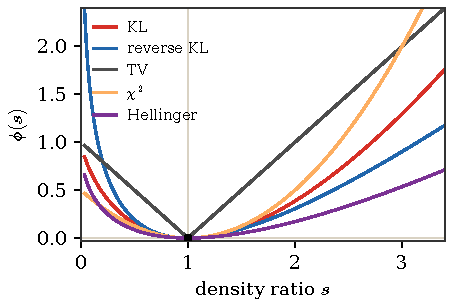
\includegraphics[width=.43\linewidth]{figures/dualnorms-phi-generators/generators.pdf} &
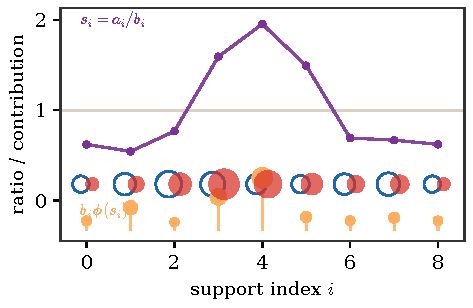
\includegraphics[width=.43\linewidth]{figures/dualnorms-phi-generators/ratio-penalties.pdf}
\end{tabular}
\caption{\emph{$\phi$-divergences through density ratios.} The left panel shows normalized generators for common divergences as functions of $s=\d\alpha/\d\beta$; all curves vanish at $s=1$ up to affine normalization. The right panel shows the discrete formula $D_\phi(a|b)=\sum_i b_i\phi(a_i/b_i)$: hollow blue circles encode $b_i$, filled red circles encode $a_i$, the violet curve gives the ratios $a_i/b_i$, and orange lollipops show local KL-type contributions.}
\index{phi-divergence}% strictindex
\index{density!ratio}% strictindex
\label{fig:dualnorms-phi-generators}
\end{figure}

\begin{rem}[$\phi$-divergences versus Bregman divergences]
\index{Bregman!divergence}% strictindex
	Except for KL-type entropies, $\phi$-divergences should not be confused with Bregman divergences. A $\phi$-divergence compares measures pointwise through the density ratio $\d\alpha/\d\beta$. It is invariant under measurable bijections and, more generally, cannot increase under a measurable coarse-graining or Markov kernel~\cite{ciszar1967information}. A Bregman divergence is generated by a convex functional on a linear space and measures first-order Taylor error. KL is special because the integral entropy $\alpha\mapsto\int \rho\log\rho$ produces a Bregman divergence whose density-ratio form is also a $\phi$-divergence.
\index{data-processing inequality}% strictindex
\index{convex!function}% strictindex
\index{phi-divergence}% strictindex
\index{density!ratio}% strictindex
\end{rem}

\paragraph{Variational dual formula.}
\index{variational dual formula}% strictindex

The following formula turns a pointwise density-ratio penalty into a dual optimization problem over test functions. It is the analogue, for $\phi$-divergences, of the Kantorovich dual formula for transport costs.
\index{dual!formula}% strictindex

\begin{proposition}[Variational representation of a $\phi$-divergence]\label{prop-phi-div-dual}
	Assume that $\Xx$ is compact and let $\al,\be\in\Mm_+(\Xx)$. Define the Legendre transform of the entropy, already extended by $+\infty$ on negative arguments, by
\index{Legendre transform}% strictindex
	\eq{
		\phi^*(s) \eqdef \sup_{r\geq0}\{sr-\phi(r)\}.
	}
	Then
	\eql{\label{eq-dual-div}
		\Divergm_\phi(\al|\be)
		=
		\sup_{f\in\Cc(\Xx)}
		\left\{\int_\Xx f\d\al-\int_\Xx\phi^*(f)\d\be\right\}.
	}
	Equivalently, the convex conjugate of $\Divergm_\phi(\cdot|\be)$ on $\Mm(\Xx)$ is
\index{Legendre transform}% strictindex
	\eql{\label{eq-legendre}
		\foralls f \in \Cc(\Xx), \quad
		\Divergm_\phi^*(f|\be) = \int_\Xx \phi^*(f(x)) \d\be(x).
	}
\end{proposition}

\begin{proof}
	First suppose that $\phi'_\infty=+\infty$. Finite divergence then forces $\al=\rho\be$ for some $\rho\geq0$, and pointwise convex duality gives
	\begin{align*}
		\Divergm_\phi^*(f|\be)
		&= \sup_{\rho\geq0}
		\int_\Xx \bigl(f(x)\rho(x)-\phi(\rho(x))\bigr)\d\be(x)\\
		&= \int_\Xx \sup_{r\geq0}\bigl(f(x)r-\phi(r)\bigr)\d\be(x)
		= \int_\Xx \phi^*(f(x))\d\be(x).
	\end{align*}
	For finite $\phi'_\infty$, the effective domain of $\phi^*$ is bounded above by $\phi'_\infty$. Hence a singular mass contributes at most $\phi'_\infty\al^\perp(\Xx)$ to the pairing, exactly matching the recession term in~\eqref{eq-phi-div}; approximation by continuous test functions recovers this value. The same conjugate formula therefore holds in general. Proposition~\ref{prop-basic-phi-divergence-properties} gives convexity and weak-* lower semicontinuity, so Fenchel--Moreau yields~\eqref{eq-dual-div}.
\end{proof}


%%%%%%%%%%%%%%%%%%%%%%%%%%%%%%%%%%%%%%%%%%%%%%%%%%%%%%%%%%%%%%%
\section{GANs via Duality}
\label{sec-gan-duality}
\index{GAN}% strictindex


GANs fit naturally into the dual viewpoint: the discriminator is a parameterized potential and the generator moves a reference measure. This section first explains the original divergence-based GAN objective, then contrasts it with integral probability metrics such as MMD and Wasserstein distances.
\index{maximum mean discrepancy}% strictindex
\index{integral probability metric}% strictindex
\index{Wasserstein!distance}% strictindex
\index{reference!measure}% strictindex

The goal is to fit a generative parametric model $\al_\th = g_{\th,\sharp} \zeta$ to empirical data $\be = \frac{1}{m}\sum_{j=1}^m \de_{y_j}$, where $\zeta \in \Mm_+^1(\Zz)$ is a fixed latent probability measure and $g_\th : \Zz \rightarrow \Xx$ is the generator, often a neural network.

\paragraph{Divergence-based adversarial losses.}
\index{adversarial!loss}% strictindex

Any $\phi$-divergence can be written in adversarial form through the dual formula~\eqref{eq-dual-div}:
\index{phi-divergence}% strictindex
\index{dual!formula}% strictindex
\eq{
	\umin{\th} \Divergm_\phi(\al_\th|\be)
	= \umin{\th} \usup{\f} \int_\Xx f(x) \d\al_\th(x) - \Divergm_\phi^*(f|\be)
	= \umin{\th} \usup{\f} \int_\Xx f(g_\th(z)) \d\zeta(z) -
	\frac{1}{m}\sum_{j=1}^m \phi^*(f(y_j)).
}
Replacing the unrestricted potential $f$ by a neural network $f_\xi$ gives the restricted saddle problem
\[
	\min_\theta\max_\xi
	\int_\Zz f_\xi(g_\theta(z))\d\zeta(z)
	-
	\frac1m\sum_{j=1}^m \phi^*(f_\xi(y_j)).
\]
For fixed $\theta$, this restriction gives a lower bound on the exact divergence unless the discriminator class is rich enough to attain the supremum. This distinction is essential for empirical data: if $\be$ is discrete and $\al_\theta$ is non-atomic, a superlinear divergence is $+\infty$, whereas its neural restricted objective can remain finite. The original vanilla GAN~\cite{GAN} corresponds, up to an additive constant and the usual reparametrization by a discriminator taking values in $(0,1)$, to the unscaled Jensen--Shannon generator $\widehat\phi_{\JS}=2\phi_{\JS}$,
\[
	\widehat\phi_{\JS}(s)=s\log s-(s+1)\log\frac{s+1}{2},
	\qquad
	\widehat\phi_{\JS}^*(u)=-\log(2-e^u),\quad u<\log2.
\]
Thus $\Divergm_{\widehat\phi_{\JS}}=2\JS^2$, consistently with the normalization above. In practice the min--max problem is solved by alternating stochastic gradient descent/ascent on $(\theta,\xi)$. Although the unrestricted maximization is concave in the function $f$, neural parametrization generally destroys concavity in $\xi$; the generator problem is likewise non-convex in $\theta$. These facts contribute to instability and mode collapse. Moreover, density-ratio losses are informative when the measures overlap but can saturate when model and data are mutually singular: $\JS^2$ reaches its maximum $\log2$ on disjoint supports.
\index{stochastic!gradient}% strictindex
\index{Jensen-Shannon divergence}% strictindex
\index{density!ratio}% strictindex

\paragraph{Dual norms and integral probability metrics.}
\index{dual!norm}% strictindex
\index{integral probability metric}% strictindex

Instead of a density-ratio divergence, one can minimize a dual norm~\eqref{eq-dual-norm-cont}, also called an integral probability metric,
\eq{
	\umin{\th} \norm{\al_\th - \be}_B
	= \umin{\th}
	\usup{\f \in B} \int_{\X} \f(x) \d(\al_\th-\be)(x)
	= \umin{\th}
	\usup{\f \in B} \int_{\Zz} \f( g_\th(z)) \d\zeta - \frac{1}{m} \sum_{j=1}^m f(y_j).
}
MMD-GANs take $B$ to be a unit ball in an RKHS~\cite{MMD-GAN}; Wasserstein GANs take $B$ to be a Lipschitz ball, following Kantorovich--Rubinstein duality~\cite{WassersteinGAN,FrognerNIPS}. The advantage is topological: for a continuous kernel on a compact space, the RKHS unit ball is uniformly bounded and equicontinuous, while the normalized Lipschitz ball is compact by Arzel\`a--Ascoli. The corresponding objectives are therefore continuous for weak convergence. They can compare singular empirical and generated measures through test functions instead of requiring pointwise density ratios. The price is that the discriminator class must be controlled geometrically, by a kernel norm, a Lipschitz constraint or a related regularization.
\index{kernel!norm}% strictindex
\index{RKHS}% strictindex
\index{maximum mean discrepancy}% strictindex
\index{Kantorovich-Rubinstein@Kantorovich--Rubinstein!duality}% strictindex
\index{discriminator class}% strictindex
\index{density!ratio}% strictindex
%

\begin{example}[Application to imitation learning]\label{ex-imitation-learning-ot}
\index{imitation learning}% strictindex
\index{reinforcement learning}% strictindex
	In imitation learning, one can compare the expert occupancy measure \(\rho_E\) and the learner occupancy measure \(\rho_\theta\) on state-action space. OT gives either a primal matching loss \(W(\rho_\theta,\rho_E)\), or a dual adversarial reward obtained from a Kantorovich potential. Thus the discriminator in an adversarial imitation method can be interpreted as a learned reward shaping the learner toward the expert distribution, exactly as the GAN discriminator above is a learned potential. Wasserstein adversarial imitation and primal Wasserstein imitation exploit this distribution-matching viewpoint while retaining the geometry of state-action space, for instance through a cost that compares nearby states and actions more mildly than distant ones~\cite{XiaoHermanWagnerZiescheEtesamiLinh2019WAIL,DadashiHussenotGeistPietquin2020PWIL}.
\end{example}

\begin{rem}[Weight clipping is only a proxy]
\index{weight clipping}% strictindex
	Wasserstein GANs originally used weight clipping, constraining $\norm{\xi}_\infty \leq 1$ as a proxy for enforcing $\f_\xi \in B = \enscond{f}{\Lip(f) \leq 1}$. The parameter box is convex, but its image through a neural-network parametrization is neither the full Lipschitz ball nor generally a convex class of functions, and optimization in the parameters remains non-concave. Clipping is therefore a practical heuristic rather than a faithful implementation of the Kantorovich--Rubinstein constraint.
\end{rem}
